%!TEX root = Main.tex
\section{Theory}

\subsection{Image}
We use the $256 \times 256$ pixel grayscale cameraman image (Figure \ref{fig:image_cameraman}). 
The image is saved in the TelosB flash as a binary file. Each pixel is represented with one byte, which gives a grayscale resolution of 256 shades.

\begin{figure}[ht!]
\centering
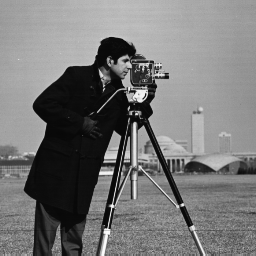
\includegraphics{cameraman}
\caption{Cameraman image used in the project.}
\label{fig:image_cameraman}
\end{figure}

\subsection{Compression}

We use three different lossy compression algorithms in this project.
They have a simple implementation and are fast to compute, but they are not very good at retaining image quality compared to e.g. JPEG which uses discrete cosine transform and Huffman coding.

Our algorithms are fast to compute since they mostly use cheap operations like bit swifting and bitwise AND/OR, and only iterates through the data once.
Lower computation time also means that the energy consumption is lower.

Our compression algorithms work by throwing away the least significant bit/bits from every byte in the image.
For instance the four bit compression takes two bytes, \texttt{aaaa\_\_\_\_} and \texttt{bbbb\_\_\_\_}, and compresses them to a single byte \texttt{aaaabbbb}, where \texttt{a}, \texttt{b} and \texttt{\_} is a bit. Using this method, the image has been compressed 50\%.


\subsubsection{One Bit Compression} % (fold)
\label{sub:one_bit_compression}

The One Bit Compression gives a compression of $\dfrac{1\ bit}{8\ bit} = 12.5\%$.
The algorithm takes 8 bytes and maps them into 7 bytes where the least significant bit, of each byte, is lost.

\subsubsection{Two bit compression} % (fold)
\label{sub:two_bit_compression}

The Two Bit Compression gives a compression of $\dfrac{2\ bit}{8\ bit} = 25\%$.
The algorithm takes 4 bytes and maps them into 3 bytes where the two least significant bits, of each byte, is lost.

\subsubsection{Four bit compression} % (fold)
\label{sub:four_bit_compression}

The Four Bit Compression gives a compression of $\dfrac{4\ bit}{8\ bit} = 50\%$.
The algorithm takes 2 bytes and maps them into 1 byte where the four least significant bits, of each byte, is lost.



